\subsection{Operational Temperature Range}
%1&2
\begin{figure}[htb]
\begin{subfigure}{.47\textwidth}
  \centering
  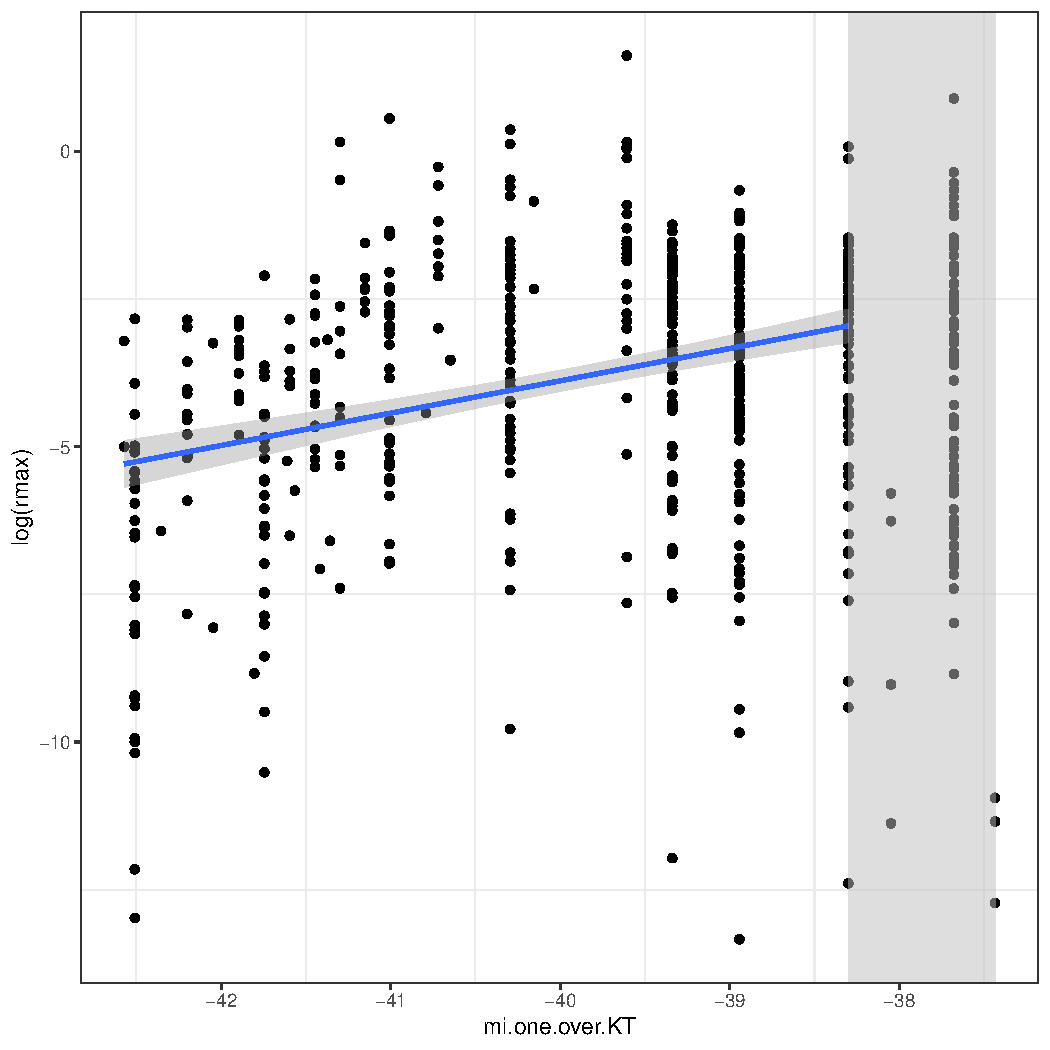
\includegraphics[width=.9\linewidth]{Plot/log_r_KT.pdf}
  \caption{$r_{max}$}
  \label{fig:log_r_KT}
\end{subfigure}%
\begin{subfigure}{.47\textwidth}
  \centering
  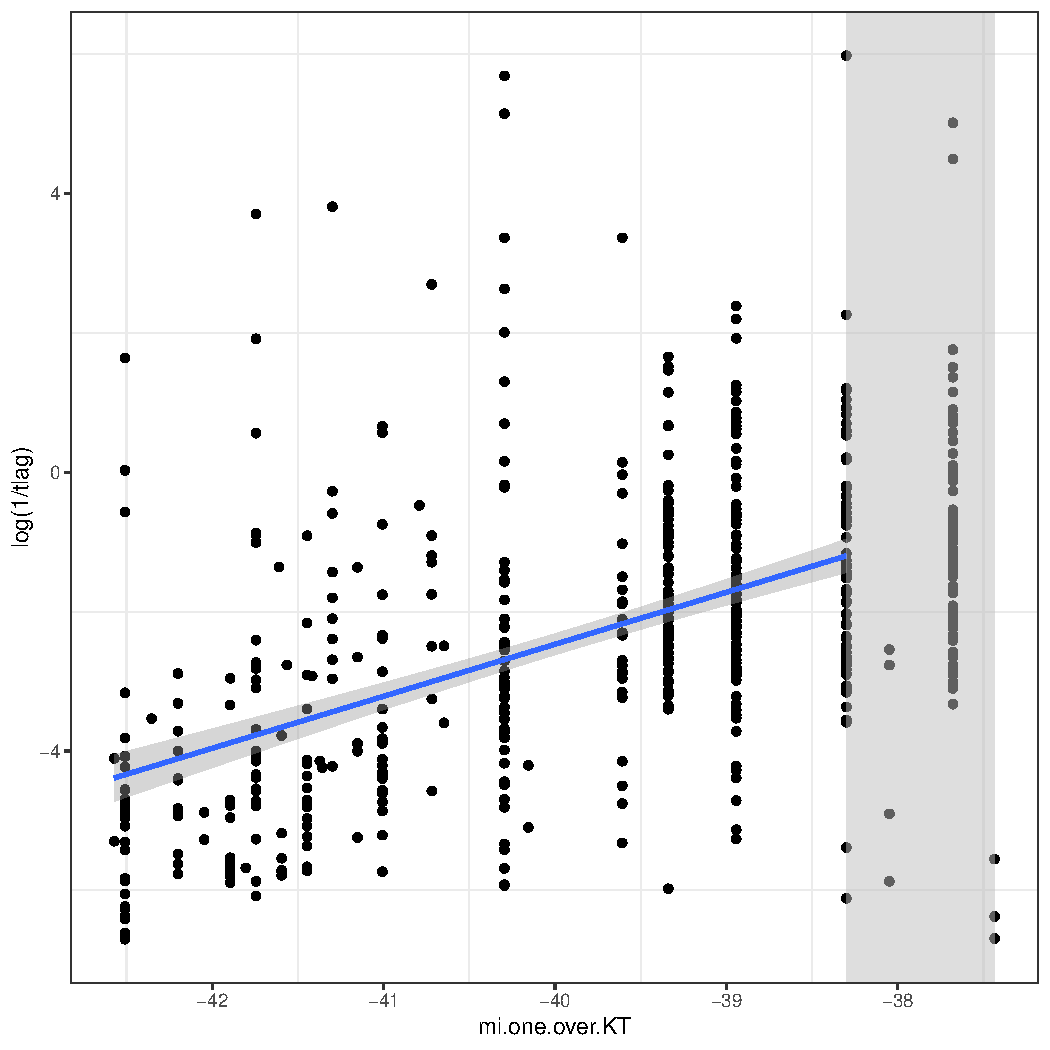
\includegraphics[width=.9\linewidth]{Plot/log_1tlag_KT.pdf}
  \caption{$t_{lag}$}
  \label{fig:log_1tlag_KT}
\end{subfigure}
\caption{Across species log of maximum growth rate ($log(r_{max})$, left) and log of lag phase growth rate($log(\frac{1}{t_{lag}})$, right) corresponding to the value of $\frac{-1}{KT}$}
\label{fig:rate_KT}
\end{figure}

%3 & 4
\begin{figure}[htb]
    \begin{subfigure}{.47\textwidth}
      \centering
      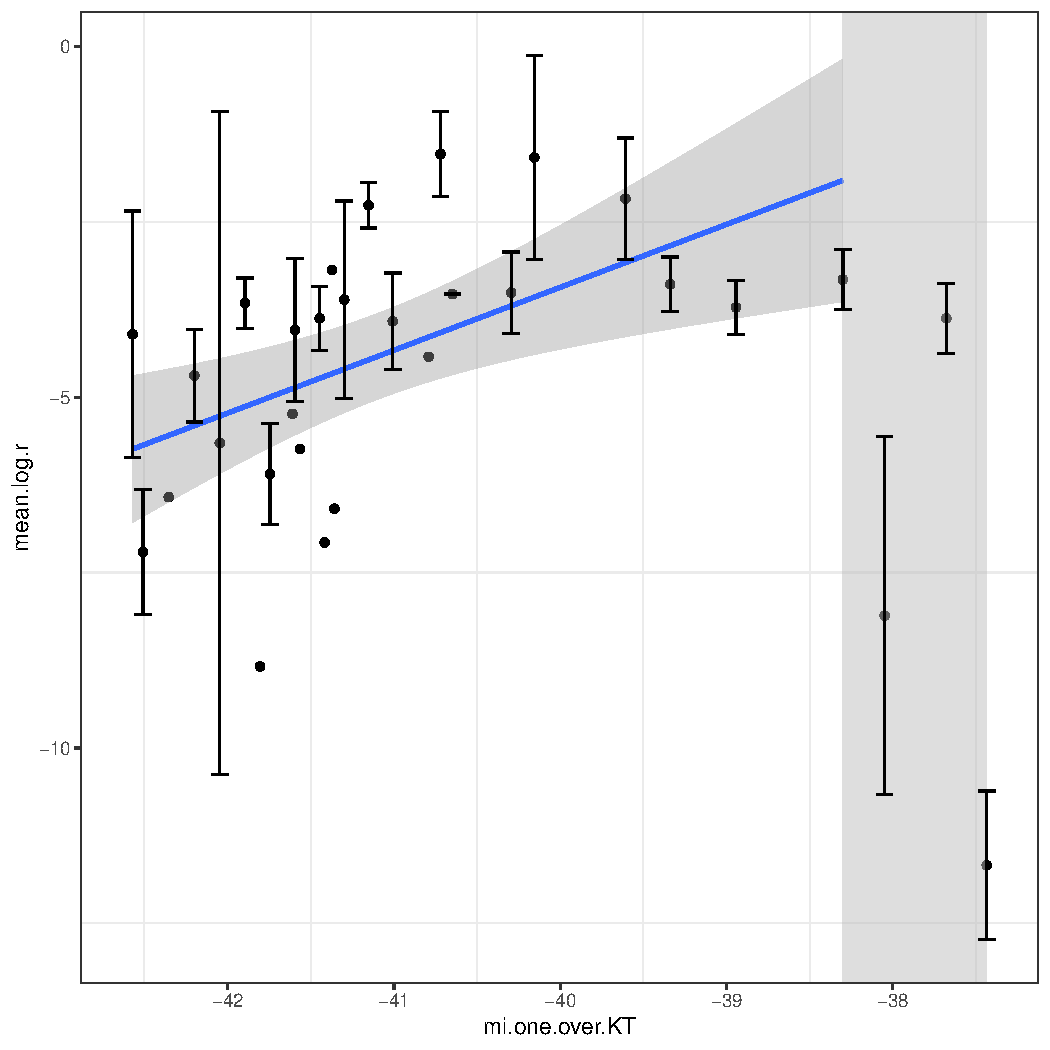
\includegraphics[width=.9\linewidth]{Plot/log_mean_r_KT.pdf}
      \caption{$r_{max}$}
      \label{fig:log_mean_r_KT}
    \end{subfigure}
    \begin{subfigure}{.47\textwidth}
      \centering
      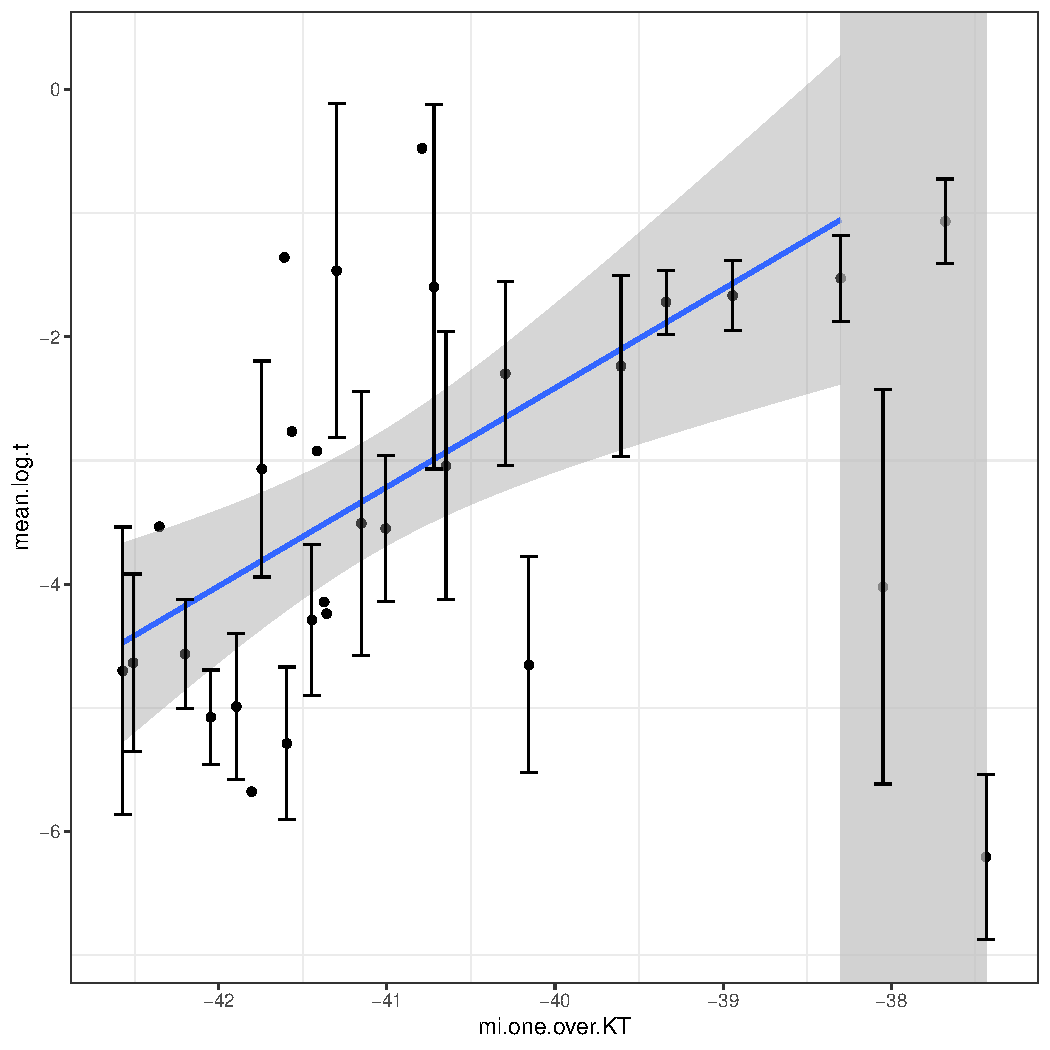
\includegraphics[width=.9\linewidth]{Plot/log_mean_tlag_KT.pdf}
      \caption{$t_{lag}$}
      \label{fig:log_mean_tlag_KT}
    \end{subfigure}
\caption{plots of across species mean log of maximum growth rate ($log(r_{max})$, left) and mean log of lag phase growth rate($log(\frac{1}{t_{lag}})$, right) corresponding to the value of $\frac{-1}{KT}$}
\label{fig:mean_rate_KT}
\end{figure}


%%% ecomp 2 plot
% figure
\begin{figure}[htb]
\begin{subfigure}{.47\textwidth}
  \centering
  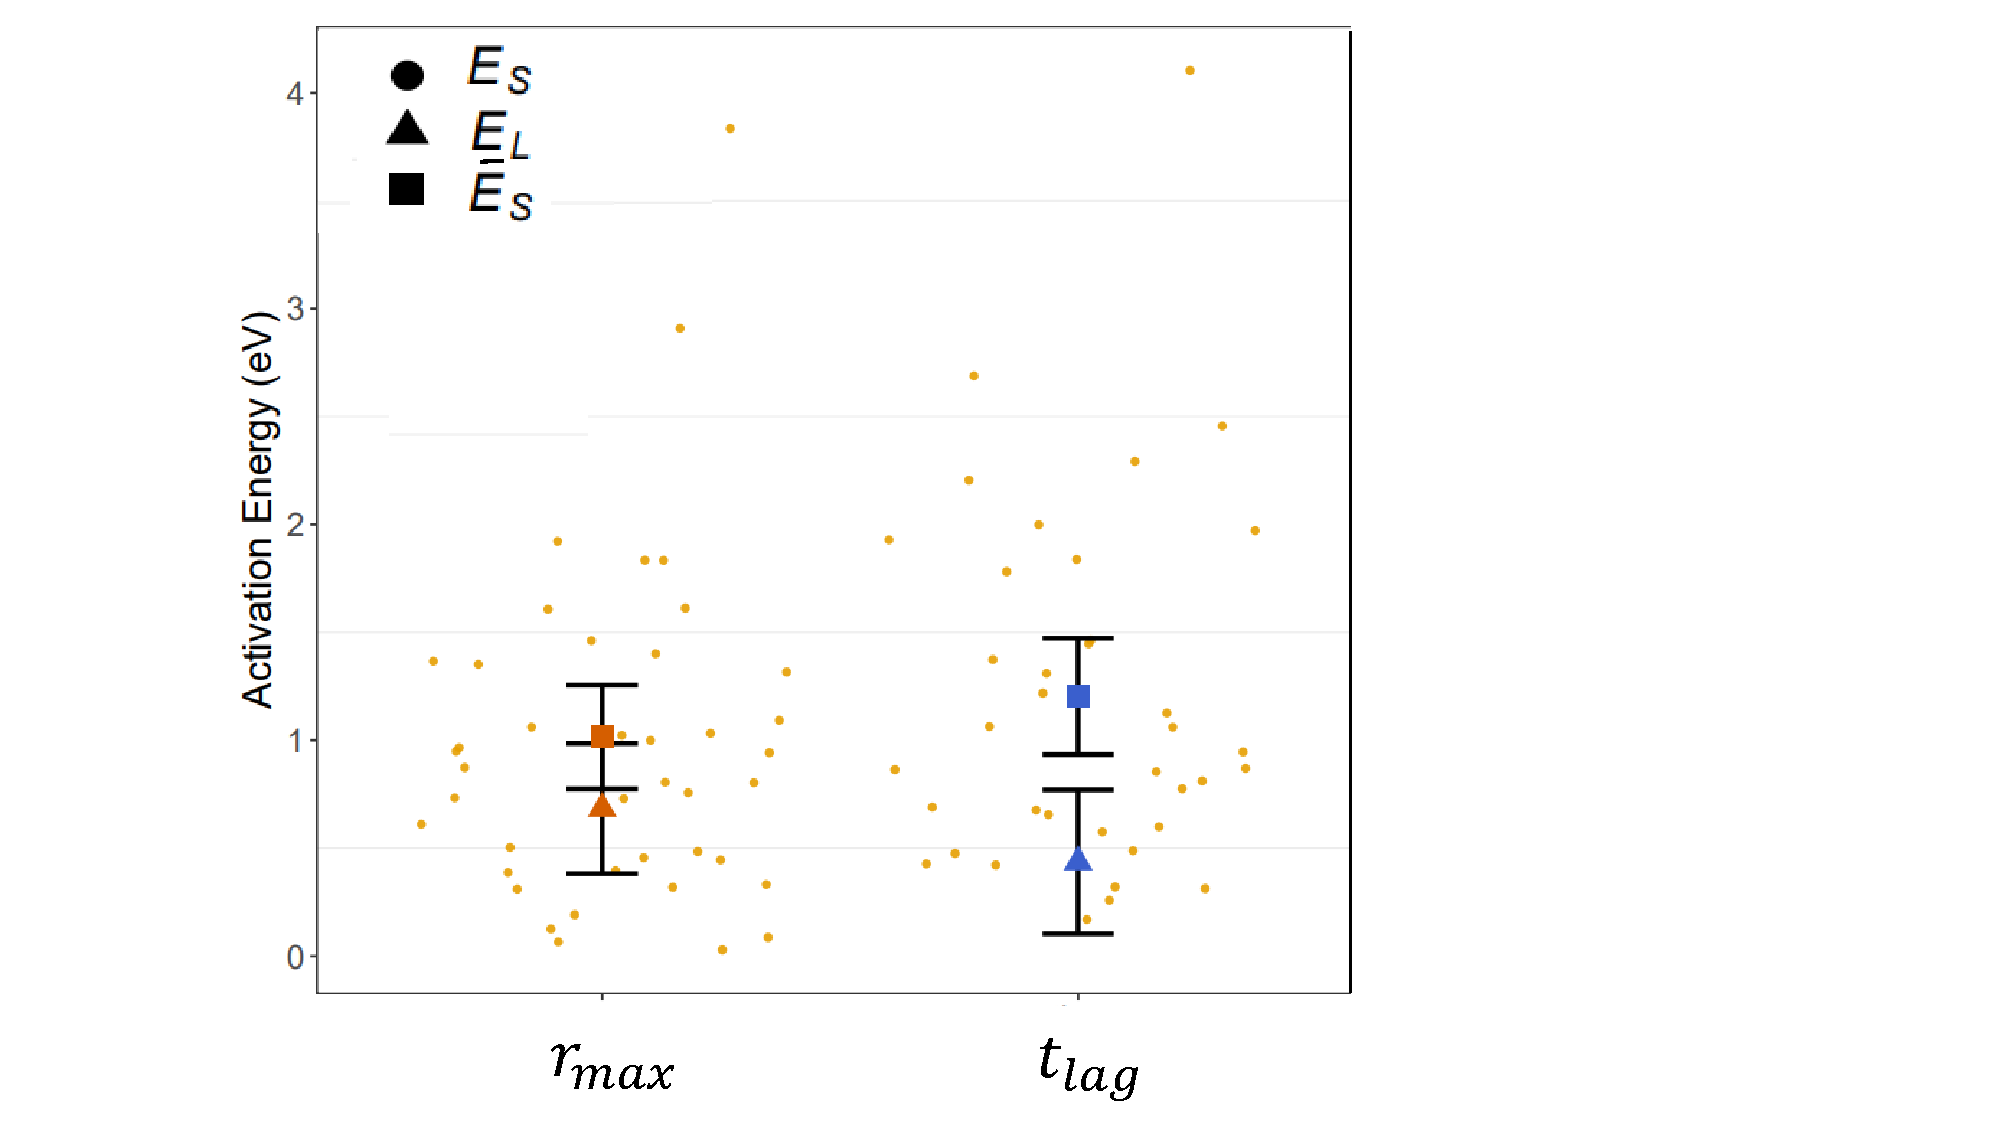
\includegraphics[width=1.5\linewidth]{Plot/E_comperasion.pdf}
  \caption{Thermal response comparison}
  \label{fig:E_comperasion}
\end{subfigure}%
\begin{subfigure}{.37\textwidth}
  \centering
  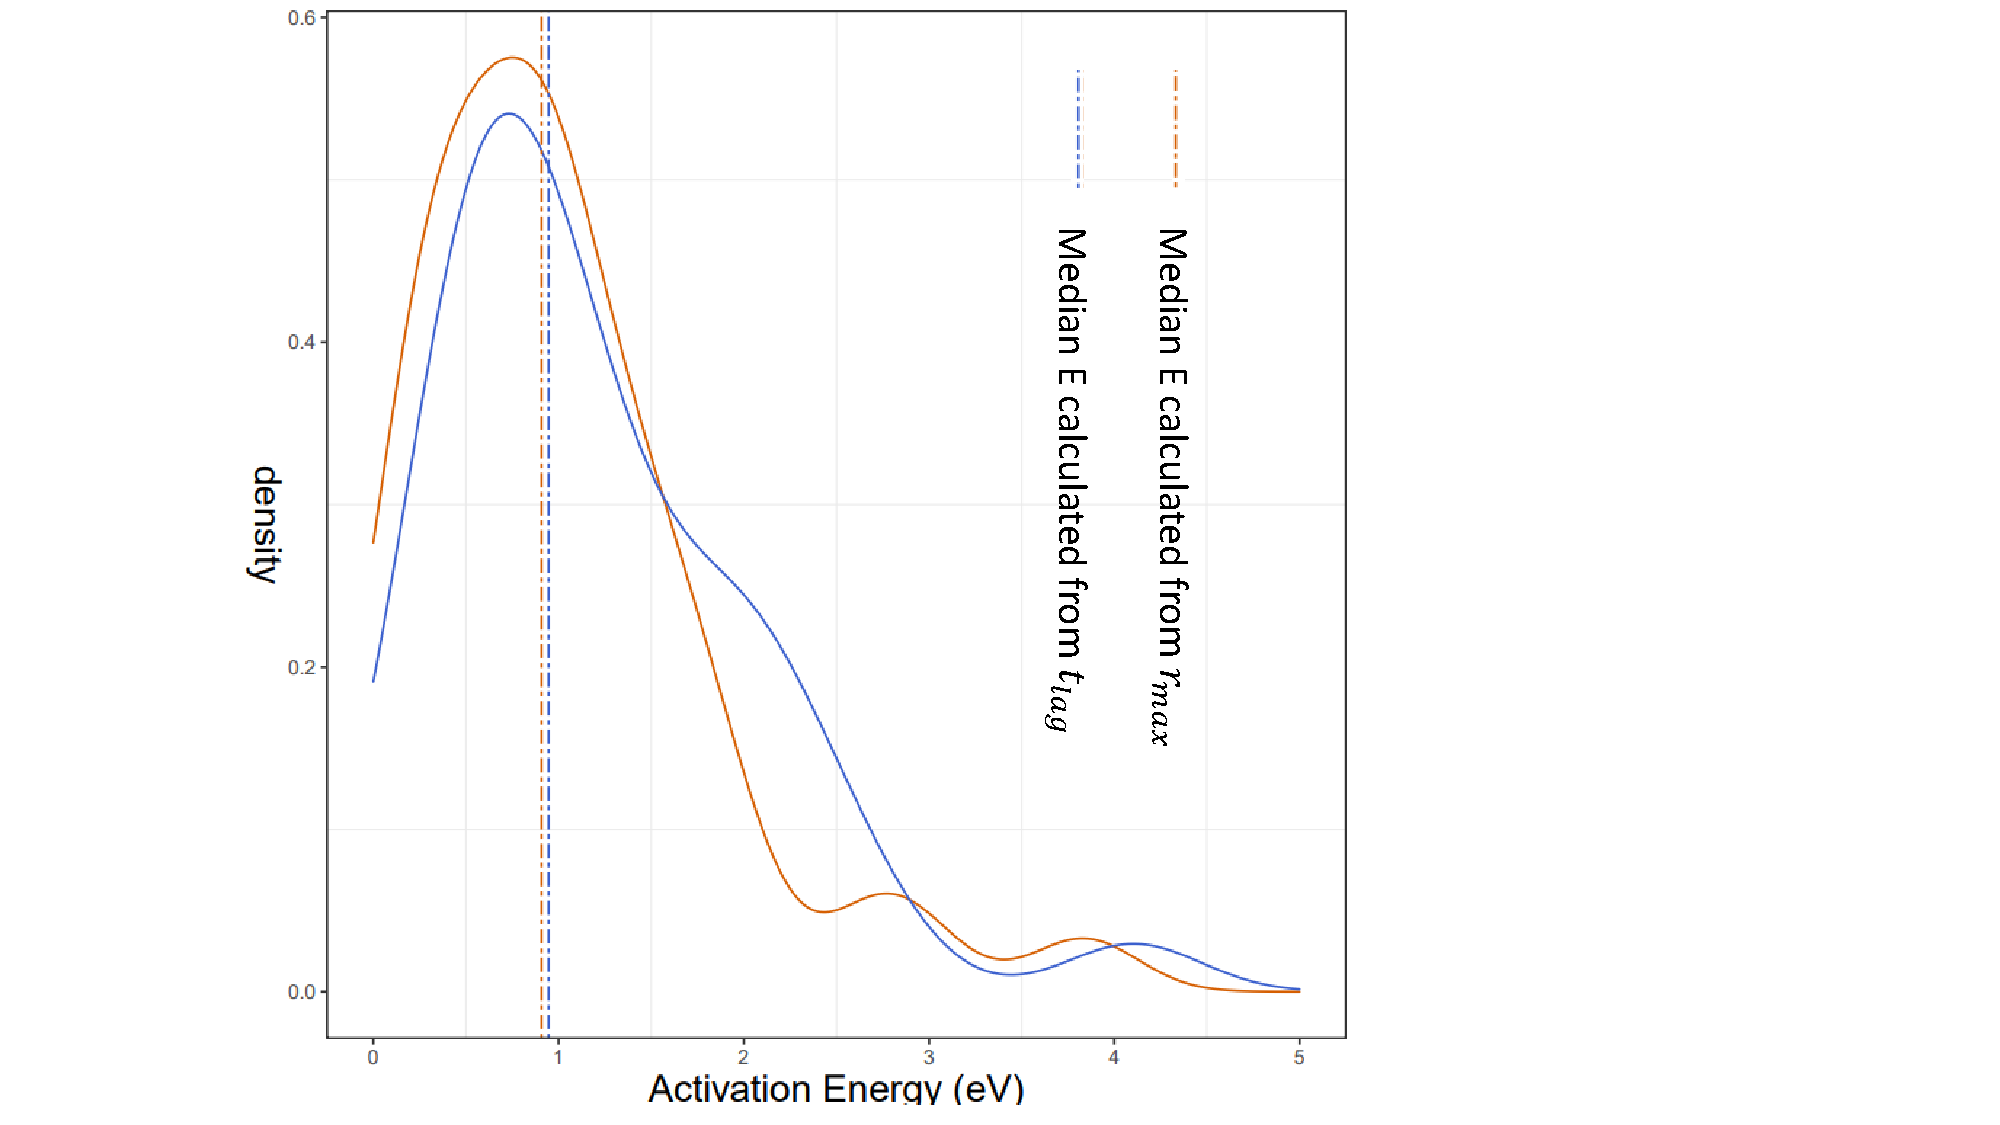
\includegraphics[angle=90, width=.99\linewidth]{Plot/E_hist.pdf}
  \caption{Short-term thermal responses.
  %, with x axis represents the estimated activation energy and y axis represents the density of species has respective activation energy value, and red bar and blue bar denote estimated from parameter $r_{max}$ and $t_{lag}$ respectively, and 
  }
  \label{fig:E_hist}
\end{subfigure}
\caption{\textbf{a} The thermal responses of each species ($E_S$, yellow dots). The mean value ($\bar{E}_{S}$, blue triangles) of them is taken as the short-term thermal responses of exponential and lag phases. The long-term thermal responses ($E_L$, orange squares) were calculated using the best performance metabolic rate parameters in each species. Both short-term and long-term thermal responses have error bars with 95\% confidence intervals.
\textbf{b} Distribution of activation energy of species estimated from exponential(red) and lag (blue) phases. The two "twodash" lines represent median activation energy value, "dotted" lines represent mean activation energy value}
\label{fig:E_comp}
\end{figure}